\documentclass[a4paper]{article}
\usepackage{fancyhdr}
\usepackage{physics}
\usepackage{graphicx}

\usepackage{subcaption}
\usepackage{floatrow}

\graphicspath{ {img/} }

\title{Meine Antwort zum erweiterten Wigner's Freund Gedankenexperiment}
\author{Jannis Naske}

\pagestyle{fancy}
\fancyhf{}
\rhead{Jannis Naske}

\begin{document}
\pagenumbering{gobble}
\maketitle
\pagenumbering{arabic}

\section*{Abstract}
In diesem Dokument schlage ich zwei mögliche Korrekturen zum erweiterten Wigner's Freund Gedankenexperiment von Renner und Frauchiger vor.
Durch diese Verbesserungen wird der Widerspruch vernichtet, und alle drei Annahmen, \textbf{(Q)}, \textbf{(C)} und \textbf{(S)}, bleiben unverletzt.

\section*{Der erste Fehler}
Im Artikel von Renner und Frauchiger wird folgendes Statement hergeleitet:
\begin{itemize}
	\item \textbf{Statement 1 by} $F_1$: ``If I get $t$, I know that $W_2$ will measure $plus$''
\end{itemize}
Der Beweis, welcher benutzt wird, ist folgender(ich lasse in diesem Dokument die doppelten Symbole weg, da dies in diesem Fall redundante Information ist):\\\\
Nachdem $F_1$ $t$ gemessen hat, setzt er den Spin für $F_2$ in die Superposition $\frac{1}{\sqrt{2}} \ket{\downarrow} + \frac{1}{\sqrt{2}} \ket{\uparrow}$.
In der Basis $\qty{\ket{+}_{L_2}, \ket{-}_{L_2}}$, mit $\ket{+}_{L_2} = \frac{1}{\sqrt{2}} \ket{\downarrow} + \frac{1}{\sqrt{2}} \ket{\uparrow}$, $\ket{-}_{L_2} = \frac{1}{\sqrt{2}} \ket{\downarrow} - \frac{1}{\sqrt{2}} \ket{\uparrow}$,
ist diese Superposition dargestellt als $\ket{+}_{L_2}$, und $W_2$ wird somit $\ket{+}_{L_2}$ messen, und die Aussage folgt.\\\\
Jedoch wurde bei diesem Beweis weggelassen, dass die Superposition durch das Messen von $W_1$ verändert wird.
Wenn $W_1$ nach Annahme $\ket{-}_{L_1} = \frac{1}{\sqrt{2}}\ket{h} + \frac{1}{\sqrt{2}}\ket{t}$ misst, geht die Superposition, nach dem Artikel,
in $\ket{-}_{L_1}\ket{\uparrow} = \frac{1}{\sqrt{2}}\ket{h}\ket{\uparrow} - \frac{1}{\sqrt{2}}\ket{t}\ket{\uparrow} = \qty(\frac{1}{\sqrt{2}} \ket{h} - \frac{1}{\sqrt{2}} \ket{t})\qty(\ket{+}_{L_2} - \ket{-}_{L_2}) = \frac{1}{2}\ket{h}\ket{+}_{L_2} - \frac{1}{2}\ket{t}\ket{+}_{L_2} - \frac{1}{2}\ket{h}\ket{-}_{L_2} + \frac{1}{2}\ket{t}\ket{-}_{L_2}$ über. Es ist also doch möglich, dass $W_2$ $\ket{t}\ket{-}_{L_2}$ misst, und Statement 1 stellt sich als falsch heraus.\\\\
Zum Schluss misst $W_2$ nach Annahme noch $\ket{-}_{L_2}$, und der Zustand geht in $\frac{1}{\sqrt{2}}\ket{t}\ket{-} - \frac{1}{\sqrt{2}}\ket{h}\ket{-} = \frac{1}{2}\ket{t}\ket{\downarrow} - \frac{1}{2}\ket{t}\ket{\uparrow} - \frac{1}{2}\ket{h}\ket{\downarrow} + \frac{1}{2}\ket{h}\ket{\uparrow}$ über.

\section*{Der zweite Fehler}
Da das Statement 1 nicht mehr gilt, verschwindet die sich widersprechende Aussage aus dem ursprünglichen Bericht. Jedoch gibt es noch ein Problem. Oben haben wir den Zustand $\frac{1}{2}\ket{t}\ket{\downarrow} - \frac{1}{2}\ket{t}\ket{\uparrow} - \frac{1}{2}\ket{h}\ket{\downarrow} + \frac{1}{2}\ket{h}\ket{\uparrow}$ als Schlusszustand hergeleitet, worauf die Korrektur des ersten Fehlers keinen Einfluss hat. Wenn aber in diesem Zustand in den Standardbasen gemessen wird, ist es möglich, den Zustand $\ket{h}\ket{\uparrow}$ zu messen. Dies scheint aber aus der Perspektive von $F_1$ nicht möglich zu sein; Wenn er $h$ misst, wird er das Qubit, dass er dann an $F_2$ weiterleitet, in den Zustand $\ket{\downarrow}$ versetzen. Ist dies ein anderer Widerspruch? Um diese Frage zu beantworten, betrachten wir zuerst ein simpleres Problem, und wenden dann unsere Erkenntnis auf das Ursprüngliche Problem an.\\\\
Der Aufbau des Experiments ist in Bild 1.1 dargestellt. $Q_1$ und $Q_2$ stellen Quantenbits dar, der Freund, $F$, befindet sich mit den Bits in einer Isolation, die dann von Wigner, $W$, gemessen wird. $Q_1$ kann die Zustände $\ket{t}$, $\ket{h}$ annehmen, und $Q_2$ $\ket{\downarrow}$, $\ket{\uparrow}$. Es werden die gleichen Messregeln wie im originalen Artikel angewendet. Der Plan läuft wie folgt ab:
\begin{itemize}
	\item \textbf{Schritt 1:} $F$ setzt $Q_1$ in eine Superposition $\frac{1}{\sqrt{2}} \ket{h} + \frac{1}{\sqrt{2}} \ket{t}$.
	\item \textbf{Schritt 2:} $F$ misst $Q_1$. Ist das Ergebnis $\ket{h}$, setzt er $Q_2$ als $\ket{\downarrow}$, sonst setzt er $Q_2$ als $\ket{\uparrow}$.
	\item \textbf{Schritt 3:} $W$ misst sein Labor in der Basis $\qty{\ket{+}, \ket{-}}$, mit $\ket{+} = \frac{1}{\sqrt{2}} \ket{h} + \frac{1}{\sqrt{2}} \ket{t}$ und $\ket{-} = \frac{1}{\sqrt{2}} \ket{h} - \frac{1}{\sqrt{2}} \ket{t}$.
\end{itemize}
Nach Schritt 2 hat das Labor von $W$ den Zustand $\frac{1}{\sqrt{2}} \ket{h}\ket{\downarrow} + \frac{1}{\sqrt{2}} \ket{t}\ket{\uparrow} = $.

\begin{figure}[!htb]
\begin{floatrow}[2]\
\ffigbox{\caption*{1.1: Situation des simplen Problems}}%
{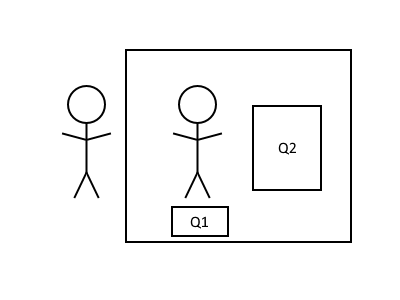
\includegraphics[width=0.5\textwidth]{a.png}}
%
%%%%%%
\ffigbox{\caption*{1.2: Wie das Problem interpretiert wird}}%
{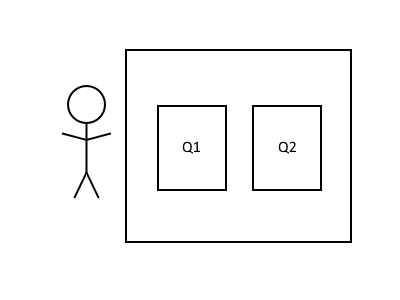
\includegraphics[width=0.5\textwidth]{b.png}}
\end{floatrow}
\end{figure}

\end{document}